\section{Cronograma para Construção da Ontologia na Aplicação}

A aplicação da ontologia no software envolvem algumas mudanças estruturais na arquitetura e
na refatoração de algumas funcionalidades, como uma busca no banco de dados por um acidente por 
exemplo. Desta forma, a equipe técnica definiu a construção da ontologia na aplicação como um projeto
separado, com cronograma próprio, integrado com o cronograma geral do projeto.
O objetivo é encarar a construção como uma mudança de requisitos, estudando o impacto e analisando
as implicações do uso da ontologia dentro da ferramenta.

\begin{figure}[h]
	\centering
	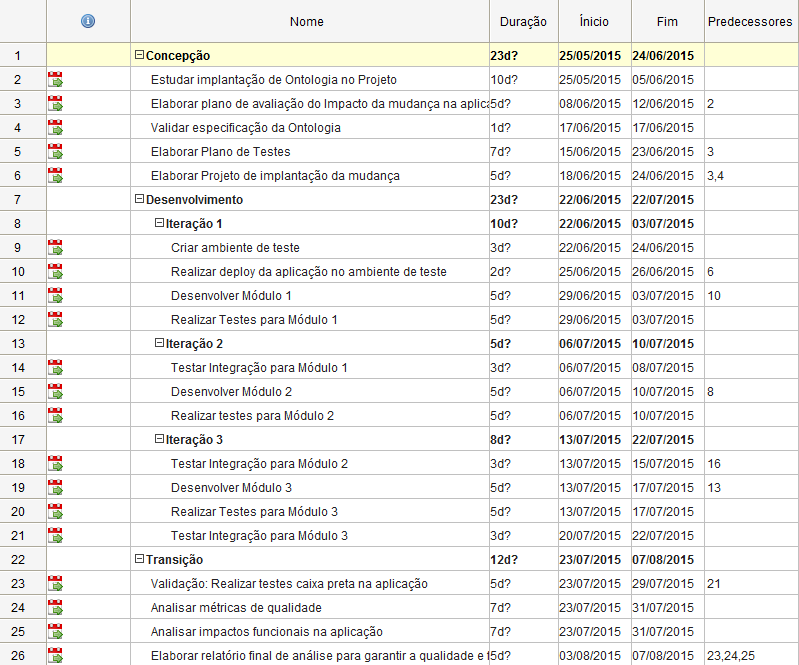
\includegraphics{Figuras/cronograma_construcao_ontologia.png}
	content...
\end{figure}

\pagebreak

Tabela – Cronograma de Construção da Ontologia na Aplicação